%******************************************************************************%
% Copyright (C) 2018  Louis Solofrizzo                                         %
%                                                                              %
% This content is considered a free software: you can redistribute it          %
% and/or modify it under the terms of the GNU General Public License as        %
% published by the Free Software Foundation, either version 3 of the License,  %
% or (at your option) any later version.                                       %
%                                                                              %
% This program is distributed in the hope that it will be useful,              %
% but WITHOUT ANY WARRANTY; without even the implied warranty of               %
% MERCHANTABILITY or FITNESS FOR A PARTICULAR PURPOSE.  See the                %
% GNU General Public License for more details.                                 %
%                                                                              %
% You should have received a copy of the GNU General Public License            %
% along with this program.  If not, see <https://www.gnu.org/licenses/>.       %
%******************************************************************************%

%******************************************************************************%
%                                                                              %
%                          KFS_4.en.tex for KFS_4                              %
%                                                                              %
%                  Created on : Wed May 25 13:27:28 2016                       %
%          Made by : Louis "Ne02ptzero" Solofrizzo <louis@ne02ptzero.me>       %
%                                                                              %
%******************************************************************************%

\documentclass{42-en}


%******************************************************************************%
%                                                                              %
%                                    Header                                    %
%                                                                              %
%******************************************************************************%
\begin{document}


                           \title{KFS\_4}
                          \subtitle{Interrupts}
                       \member{Louis Solofrizzo}{louis@ne02ptzero.me}
                        \member{42 Staff}{pedago@42.fr}

\summary {
	Interrupts, signals and fun.
}

\maketitle

\tableofcontents

%******************************************************************************%
%                                                                              %
%                                  Foreword                                    %
%                                                                              %
%******************************************************************************%
\chapter{Foreword}
	\centerline{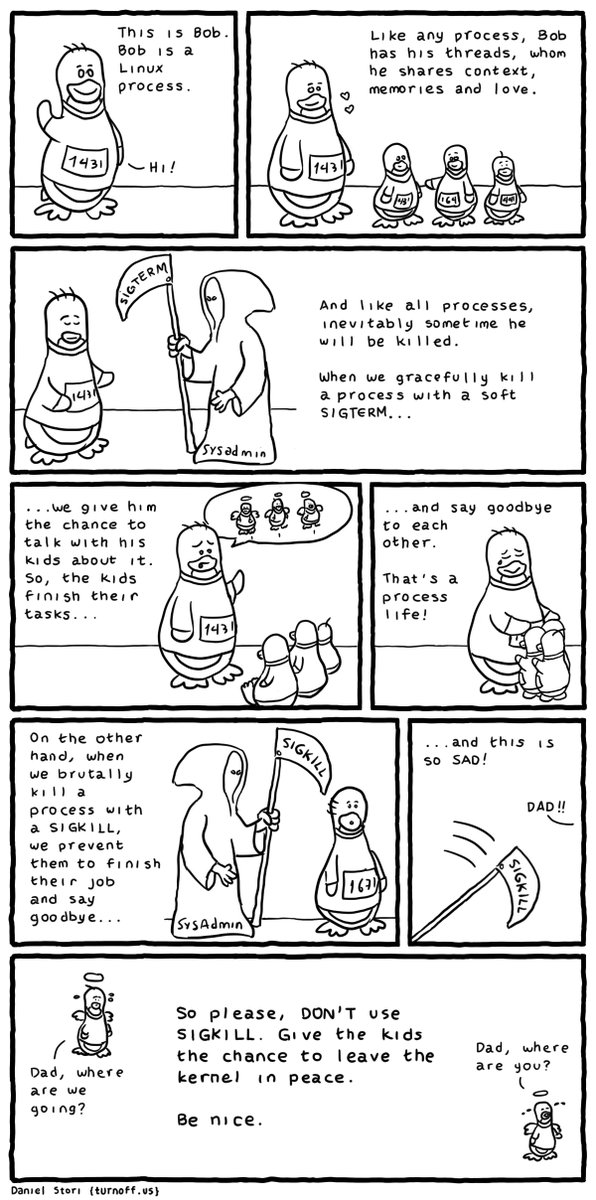
\includegraphics[width=10cm]{./lol.jpg}}


%******************************************************************************%
%                                                                              %
%                                 Introduction                                 %
%                                                                              %
%******************************************************************************%
\chapter{Introduction}
	Finally, we get to work with memory ! Let's do some work to integrate processuses.\\
	A kernel needs interrupts. Let's see why:
	\section{Interrupts}
	\begin{quotation}
		\textit{A Kernel uses a lot of different pieces of hardware to
          perform many different tasks. The video device drives the
          monitor, the IDE device drives the disks and so on. You
          could drive these devices synchronously, that is you could
          send a request for some operation (say writing a block of
          memory out to disk) and then wait for the operation to
          complete. That method, although it would work, is very
          inefficient and the operating system would spend a lot of
          time “busy doing nothing” as it waited for each operation to
          complete. A better, more efficient, way is to make the
          request and then do other, more useful work and later be
          interrupted by the device when it has finished the
          request. With this scheme, there may be many outstanding
          requests to the devices in the system all happening at the
          same time.}

	\end{quotation}
	The quote above is from
    \href{http://www.tldp.org/LDP/tlk/dd/interrupts.html}{TLDP}
    (s/Linux/A Kernel/g). A really good piece of paper to read to
    understand how interrupts work and how Linux handle them.
	\section{IDT}
	As you can see, Interrupts are perfect for the Kernel to help it
    communicate with the Hardware layer. Actually, this method is so
    good, we use it for Signals, Execeptions, Software and Hardware.\\
	To do so, we need to declare a Interrupts Descriptor Table. Let's
    see how it looks like:
	\begin{quotation}
		\textit{The Interrupt Descriptor Table (IDT) is a data
          structure used by the x86 architecture to implement an
          interrupt vector table.  The IDT is used by the processor to
          determine the correct response to interrupts and
          exceptions.}
	\end{quotation}
	Note: as mentionned above, this method is suitable only for x86
    architecture.\\
    In other words, the IDT is an interface built to
    ease communications between the Kernel and the Hardware. It
    supports the following:
	\begin{center}
		\begin{tabular}{| c | c |}
		\hline
		\textbf{INT\_NUM} & \textbf{Short Description} \\ \hline
		0x00 & Division by Zero\\ \hline
		0x01 & Debugger\\ \hline
		0x02 & NMI\\ \hline
		0x03 & Breakpoint\\ \hline
		0x04 & Overflow\\ \hline
		0x05 & Bounds\\ \hline
		0x06 & Invalid Opcode\\ \hline
		0x07 & Coprocessor not available\\ \hline
		0x08 & Double fault\\ \hline
		0x09 & Coprocessor Segment Overrun (386 or earlier only)\\ \hline
		0x0A & Invalid Task State Segment\\ \hline
		0x0B & Segment not present\\ \hline
		0x0C & Stack Fault\\ \hline
		0x0D & General protection fault\\ \hline
		0x0E & Page fault\\ \hline
		0x0F & reserved\\ \hline
		0x10 & Math Fault\\ \hline
		0x11 & Alignment Check\\ \hline
		0x12 & Machine Check\\ \hline
		0x13 & SIMD Floating-Point Exception\\ \hline
		\end{tabular}
	\end{center}
	Does it ring a bell for you ?

\newpage
%******************************************************************************%
%                                                                              %
%                                  Goals                                       %
%                                                                              %
%                                                                              %
%******************************************************************************%
\chapter{Goals}

	Once you're done with this project, you will have a complete interface to
	handle interruptions. It goes like that:

	\begin{itemize}\itemsep1pt
		\item 	Hardware Interrupts
		\item 	Software Interrupts
		\item	A Interrupts Descriptor Table
		\item	Sigal handling and scheduling
		\item	Global Panic Fault handling
	\end{itemize}
	Something above all, you will have to code proper panic \& exiting
    system commands, which include:
	\begin{itemize}\itemsep1pt
		\item	Registers cleaning
		\item	Stack saving
	\end{itemize}
	Good luck ! 

\newpage
%******************************************************************************%
%                                                                              %
%                             General instructions                             %
%                                                                              %
%******************************************************************************%
\chapter{General instructions}
	\section{Code and Execution}
		\subsection{Emulation}
		The following part is not mandatory, you're free to use any
        virtual manager you want to, however, I suggest you to use
        \texttt{KVM}, standing for \texttt{Kernel Virtual Manager}. It
        has advanced execution and debugs functions.  All of the
        examples below will use \texttt{KVM}.
		\subsection{Language}
			You're not forced to code in \texttt C language, you're free
            o use any language you want for these projects.\\

			Just keep in mind that not all languages are kernel
            friendly. You could code a kernel in \texttt{Javascript},
            but are you sure it's a good idea ?\\

            Also, the major part of the documentation is in
            \texttt{C}, you'll have to translate it to the language
            you've chosen.\\

			Furthermore, not all of a language features can be used in a
			basic kernel. For exapmle: \texttt{C++} :\\
			This language uses 'new' to make allocation, class and
            structures declaration, but in your kernel, you don't have
            a memory interface (yet), so these are useless for now.\\

			Proper languages for this could be \texttt{C},
			like \texttt{C++}, \texttt{Rust}, \texttt{Go}, etc.
			You can even code an entire kernel in \texttt{ASM} !\\
			\begin{center}
			  
\includegraphics[width=8cm]{choose.jpg}
			\end{center}

\newpage


	\section{Compilation}
		\subsection{Compilers}
			Again, you're free in the choice of the compiler. I am
            personally using \texttt{gcc} and \texttt{nasm}. You must
            render a turn in a Makefile.
		\subsection{Flags}
			In order, to boot your kernel without any dependencies,
            you must compile your code with the following flags (adapt
            them to the chosen language; those are for \texttt{C++}
            examples):
			\begin{itemize}\itemsep1pt
				\item \texttt{-fno-builtin}
				\item \texttt{-fno-exception}
				\item \texttt{-fno-stack-protector}
				\item \texttt{-fno-rtti}
				\item \texttt{-nostdlib}
				\item \texttt{-nodefaultlibs}
			\end{itemize}
			Pay attention to \texttt{-nodefaultlibs} and
            \texttt{-nostdlib}.  Your Kernel will be compiled on a
            host system, but cannot be linked to any existing library
            on it. Otherwise it won't execute.
	\section{Linking}
		You can't use any existing linker to link your kernel.  As
        specified above, it won't boot. You must create one.  Be
        carefull, you \texttt{CAN} use the 'ld' binary available on
        your host, but you \texttt{CANNOT} use the .ld file.
	\section{Architecture}
		The \texttt{i386} (x86) architecture is mandatory (thanks me
        later).
	\section{Documentation}
		A lot of documention is available, some is good, some is not.
		In my opinion, \texttt{\href{http://wiki.osdev.org/Main_Page}
		{OSDev}} wiki is one of the best.
	\section{Base code}
		In this part, you can either use your exisiting \texttt{KFS}
        code and improve it, or just re-build it from scratch. Your
        call !

\newpage
%******************************************************************************%
%                                                                              %
%                             Mandatory part                                   %
%                                                                              %
%******************************************************************************%
\chapter{Mandatory part}
	You will have to implement the following:
	\begin{itemize}\itemsep1pt
		\item Create an Interrupts Descriptor Table, fill it and register it
		\item A signal-callback system on your Kernel API
		\item An interface to schedule signals
		\item An interface to clean registers before a panic / halt
		\item An interface to save the stack before a panic
	\end{itemize}
	When you're done with all of that, you'll have to implement a IDT
    keyboard handling system.


\newpage
%******************************************************************************%
%                                                                              %
%                                 Bonus part                                   %
%                                                                              %
%******************************************************************************%
\chapter{Bonus part}

	It has not been said, but syscalls are also handled by the IDT.
    You can't implement them now (No processus / Execution), but a
    good start could be coding the base functions for it, it could
    save you some work.\\
	Also, you can add some features to the keyboard handler, for
    example multi layouts (qwerty, azerty), base functions like
    get\_line (just like read: waits for characters and return them
    when \textbackslash n is pressed).

\newpage
%******************************************************************************%
%                                                                              %
%                           Turn-in and peer-evaluation                        %
%                                                                              %
%******************************************************************************%
\chapter{Turn-in and peer-evaluation}

	Turn your work into your \texttt{GiT} repository, as usual.
	Only the work present on your repository will be graded in defense.\\

	Your work must contain your code, a Makefile and a basic virtual
    image for your kernel.\\

	Side note about the image, it's useless to the kernel for now, 
	SO THERE IS NO NEED FOR IT TO BE SIZED LIKE AN ELEPHANT.




%******************************************************************************%
\end{document}
